% Asset ID: FAS2PoissonDistributionTikZ-001
% Topic ID: FAS2PoissonDistribution
% Related lesson section: Section 8.3 and Section 9
% Source: FS1-Chp2-PoissonDistribution.pdf and transcripts.md
% Purpose: Discrete probability bar chart for X ~ Po(5), with P(X=8) highlighted.
\documentclass[tikz,border=8pt]{standalone}
\usepackage{pgfplots}
\pgfplotsset{compat=1.18}
\definecolor{Canvas}{HTML}{FAF9F6}
\definecolor{Panel}{HTML}{FFFFF0}
\definecolor{LineSoft}{HTML}{E5E5EA}
\definecolor{AccentGold}{HTML}{D4AF37}
\definecolor{AccentDeep}{HTML}{C5A059}
\definecolor{TextInk}{HTML}{2C2C2E}
\definecolor{SoftPink}{HTML}{FBEFEF}
\begin{document}
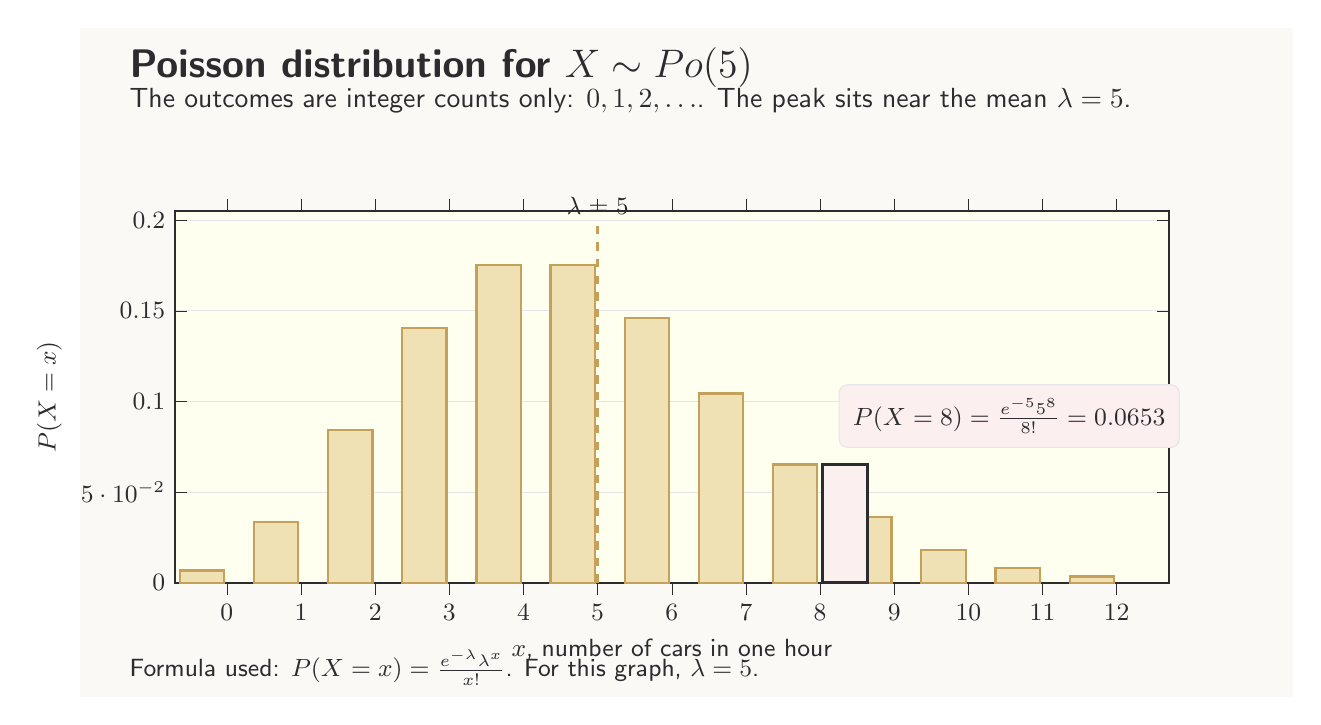
\begin{tikzpicture}
\fill[Canvas] (-1.2,-1.45) rectangle (14.2,7.05);
\node[anchor=west,text=TextInk,font=\sffamily\bfseries\Large] at (-0.7,6.55){Poisson distribution for \(X\sim\operatorname{Po}(5)\)};
\node[anchor=west,text=TextInk,font=\sffamily\normalsize] at (-0.7,6.12){The outcomes are integer counts only: \(0,1,2,\ldots\). The peak sits near the mean \(\lambda=5\).};
\begin{axis}[ybar,bar width=16pt,width=14.2cm,height=6.3cm,xmin=-0.7,xmax=12.7,ymin=0,ymax=0.205,axis background/.style={fill=Panel},axis line style={draw=TextInk,line width=0.7pt},tick style={draw=TextInk},major grid style={draw=LineSoft,line width=0.4pt},ymajorgrids=true,xlabel={\(x\), number of cars in one hour},ylabel={\(P(X=x)\)},xlabel style={font=\sffamily\small,text=TextInk},ylabel style={font=\sffamily\small,text=TextInk},tick label style={font=\sffamily\small,text=TextInk},xtick={0,1,2,3,4,5,6,7,8,9,10,11,12},ytick={0,0.05,0.10,0.15,0.20},clip=false]
\addplot[fill=AccentGold!38,draw=AccentDeep,line width=0.8pt] coordinates {(0,0.0067379)(1,0.0336897)(2,0.0842243)(3,0.1403739)(4,0.1754674)(5,0.1754674)(6,0.1462228)(7,0.1044449)(8,0.0652780)(9,0.0362656)(10,0.0181328)(11,0.0082422)(12,0.0034342)};
\addplot[fill=SoftPink,draw=TextInk,line width=1pt] coordinates {(8,0.0652780)};
\node[anchor=west,fill=SoftPink,draw=LineSoft,rounded corners=3pt,text=TextInk,font=\sffamily\small,inner sep=5pt] at (axis cs:8.25,0.092){\(P(X=8)=\frac{e^{-5}5^8}{8!}=0.0653\)};
\draw[AccentDeep,line width=1pt,dashed] (axis cs:5,0) -- (axis cs:5,0.198);
\node[anchor=south,text=TextInk,font=\sffamily\small] at (axis cs:5,0.198){\(\lambda=5\)};
\end{axis}
\node[anchor=west,text=TextInk,font=\sffamily\small] at (-0.7,-1.08){Formula used: \(P(X=x)=\frac{e^{-\lambda}\lambda^x}{x!}\). For this graph, \(\lambda=5\).};
\end{tikzpicture}
\end{document}
